% \documentclass[a4paper,12pt]{article} 
% \usepackage[T2A]{fontenc}
% \usepackage[utf8]{inputenc}
% \usepackage[english,russian]{babel}
% \usepackage{graphicx}
% \usepackage{wrapfig}
% \usepackage{mathtext} 				% русские буквы в фомулах
% \usepackage{amsmath,amsfonts,amssymb,amsthm,mathtools} % AMS
% \usepackage{icomma} % "Умная" запятая: $0,2$ --- число, $0, 2$ --- перечисление
% \usepackage{capt-of}
% \usepackage{appendix}
% \usepackage{multirow}
% \usepackage{hyperref}
% \usepackage{floatrow}
% \usepackage[margin=0.7in]{geometry}
% \usepackage{multirow}
% \usepackage{graphicx}
% \usepackage[utf8x]{inputenc} % указать кодировку русского текста

% \usepackage{fancyhdr}
% \pagestyle{fancy}
% \usepackage{graphicx}
% \usepackage{float}
% \graphicspath{{pictures/}}
% \DeclareGraphicsExtensions{.pdf,.png,.jpg}
% \usepackage{tocloft}
% \usepackage[T2A]{fontenc}
% \usepackage{capt-of}
% \usepackage[T2A]{fontenc}
% \usepackage[utf8]{inputenc}
% \usepackage[english,russian]{babel}
% \usepackage{graphicx}
% \usepackage{wrapfig}
% \usepackage{mathtext} % русские буквы в фомулах
% \usepackage{amsmath,amsfonts,amssymb,amsthm,mathtools} % AMS
% \usepackage{icomma} % "Умная" запятая: $0,2$ —- число, $0, 2$ —- перечисление
% \usepackage{capt-of}
% \usepackage{appendix}
% \usepackage{multirow}
% \usepackage{hyperref}
% \usepackage{multicol} % Несколько колонок
% \usepackage{gensymb}


% \graphicspath{ {images/} }
% \usepackage{multicol}
% \setlength{\columnsep}{2cm}


% \renewcommand{\cftsecleader}{\cftdotfill{\cftdotsep}}
% \begin{document} 
%  \begin{titlepage}
% \begin{center}
% \hfill \break
% Министерство науки и высшего образования Российской Федерации\\
% ФЕДЕРАЛЬНОЕ ГОСУДАРСТВЕННОЕ АВТОНОМНОЕ ОБРАЗОВАТЕЛЬНОЕ\\ 
% УЧРЕЖДЕНИЕ ВЫСШЕГО ОБРАЗОВАНИЯ\\ 
% «МОСКОВСКИЙ ФИЗИКО-ТЕХНИЧЕСКИЙ ИНСТИТУТ\\ 
% (НАЦИОНАЛЬНЫЙ ИССЛЕДОВАТЕЛЬСКИЙ УНИВЕРСИТЕТ)»\\
% (МФТИ)\\
% \hfill \break
% \hfill \break
% \hfill \break
% \hfill \break
% \hfill \break
% \hfill \break
% \hfill \break
% \hfill \break
% \hfill \break
% \hfill \break
% \hfill \break
% КАФЕДРА ВАКУУМНОЙ ЭЛЕКТРОНИКИ\\
% \hfill \break
% ОТЧЕТ\\
% ПО ЛАБОРАТОРНОЙ РАБОТЕ\\
% \hfill \break
% ЭЛЕКТРОННО-ОПТИЧЕСКИЙ ПРЕОБРАЗОВАТЕЛЬ\\
% \end{center}
% \hfill \break
% \hfill \break
% \hfill \break
% \hfill \break
% \hfill \break
% \hfill \break
% \hfill \break
% \hfill \break
% \begin{tabular}{ccc}
% Работу выполнили студенты:  & \underline{\hspace{5cm}}&  \\\\
% группы Б04-004& &   \\\\
%  & &  \\\\
% Работу принял, оценка & \underline{\hspace{5cm}} &  \\\\
% \end{tabular}
% \hfill \break
% \hfill \break
% \begin{center} Долгопрудный 2022 
% \end{center}
% \end{titlepage}

\documentclass[a4paper,12pt]{article} 
\usepackage[T2A]{fontenc}			
\usepackage[utf8]{inputenc}			
\usepackage[english,russian]{babel}	
\usepackage{amsmath,amsfonts,amssymb,amsthm,mathrsfs,mathtools} 
\usepackage[colorlinks, linkcolor = blue]{hyperref}
\usepackage[left=2cm,right=2cm,top=2cm,bottom=3cm,bindingoffset=0cm]{geometry}
\usepackage{subfig}
\usepackage{graphicx}
\usepackage{wrapfig}
\usepackage{multirow}
\usepackage{xcolor}
\date{\today}

\begin{document}

\begin{titlepage}
\begin{center}
    {\large МОСКОВСКИЙ ФИЗИКО-ТЕХНИЧЕСКИЙ ИНСТИТУТ (НАЦИОНАЛЬНЫЙ ИССЛЕДОВАТЕЛЬСКИЙ УНИВЕРСИТЕТ)}
\end{center}
\begin{center}
    {\large Кафедра вакуумной электроники}
\end{center}


    \vspace{1.5cm}

\begin{center}
    
\includegraphics[width=0.4\linewidth]{hv_full.png}
\end{center}
\vspace{0.01cm}
{\Large
\begin{center}
    {\bf
        Отчёт по лабораторной работе\\
        Электронно-оптический преобразователь
    }
\end{center}
}
\vspace{2cm}
\begin{flushright}
{
    \Large Выполняли студенты:\\ 
    \vspace{4mm}
    Наталья Плюскова (Б04-004),\\
    Артём Логинов (Б04-005) \\
}
\end{flushright}
\vfill
\begin{center}
    Долгопрудный, 2022
\end{center}
\end{titlepage}

\newpage


\section*{Аннотация} В данной работе требовалось построить графики зависимостей токов на элементах ЭОП от напряжений на этих же элементах, сделать некоторые выводы о характере зависимости, при этом проследить за изменением картины. Также необходимо было пронаблюдать изменение яркости при помещении в схему светофильтров.


\section*{Теоретические сведения}
\textbf{Электронно-оптический преобразователь} - вакуумный фотоэлектронный прибор для преобразования невидимого глазом изображения (в ближнем инфракрасном, ультрафиолетовом или рентгеновском спектре) в видимое для усиления яркости видимого изображения. 

Простейший ЭОП представляет собой короткий стеклянный цилиндр. На одном его торце изнутри напылён фотокатод из вещества с малой работой выхода, то есть легко ионизирующегося под действием света. На другом торце напылён люминофор, то есть вещество, светящееся под ударами электронов. Специальная система электродов обеспечивает ускорение (то есть увеличение энергии) и размножение электронов на пути от фотокатода к люминофору. Для нормальной работы на эти электроды подаются определённые напряжения, вырабатываемые источником питания ЭОП.

В качестве усилителей электронных потоков в современных ЭОП используется микроканальная пластина.
\begin{center}
    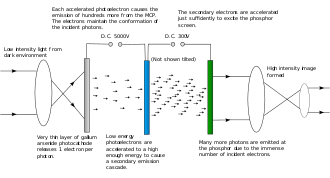
\includegraphics[scale = 1]{эоп.png}
    \captionof{figure}{Схема работы ЭОП}
\end{center}

\indent\textbf{Микроканальная пластина} - часть электровакуумных приборов, предназначена для усиления первичного потока электронов, имеющего некоторое пространственное распределение интенсивности. Принцип усиления основан на явлении вторичной электронной эмиссии при взаимодействии электронов возникающей электронной лавины с внутренними стенками каналов МКП.

По принципу действия близка к фотоэлектронным умножителям, но так как усиление фототока происходит во многих микроскопических каналах, обеспечивает пространственное разрешение распределения в потоке первичных электронов.

Когда налетающий электрон попадает в канал, то из стенки канала выбиваются вторичные электроны, которые ускоряются электрическим полем вдоль канала, которое создается приложением напряжения между стенками МКП. 

Вторичные электроны летят, пока не попадут на стенку, выбивая еще большее количество вторичных электронов. Процесс повторяется много раз, формируя электронную лавину.

\begin{center}
    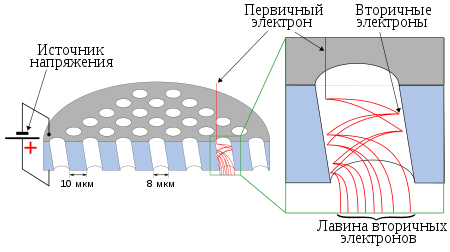
\includegraphics[scale = 0.8]{микроканальная пластина.png}
    \captionof{figure}{Схема работы микроканальной пластины}
\end{center}

\section*{Экспериментальной установка}
\begin{figure}[h!]
    \centering
    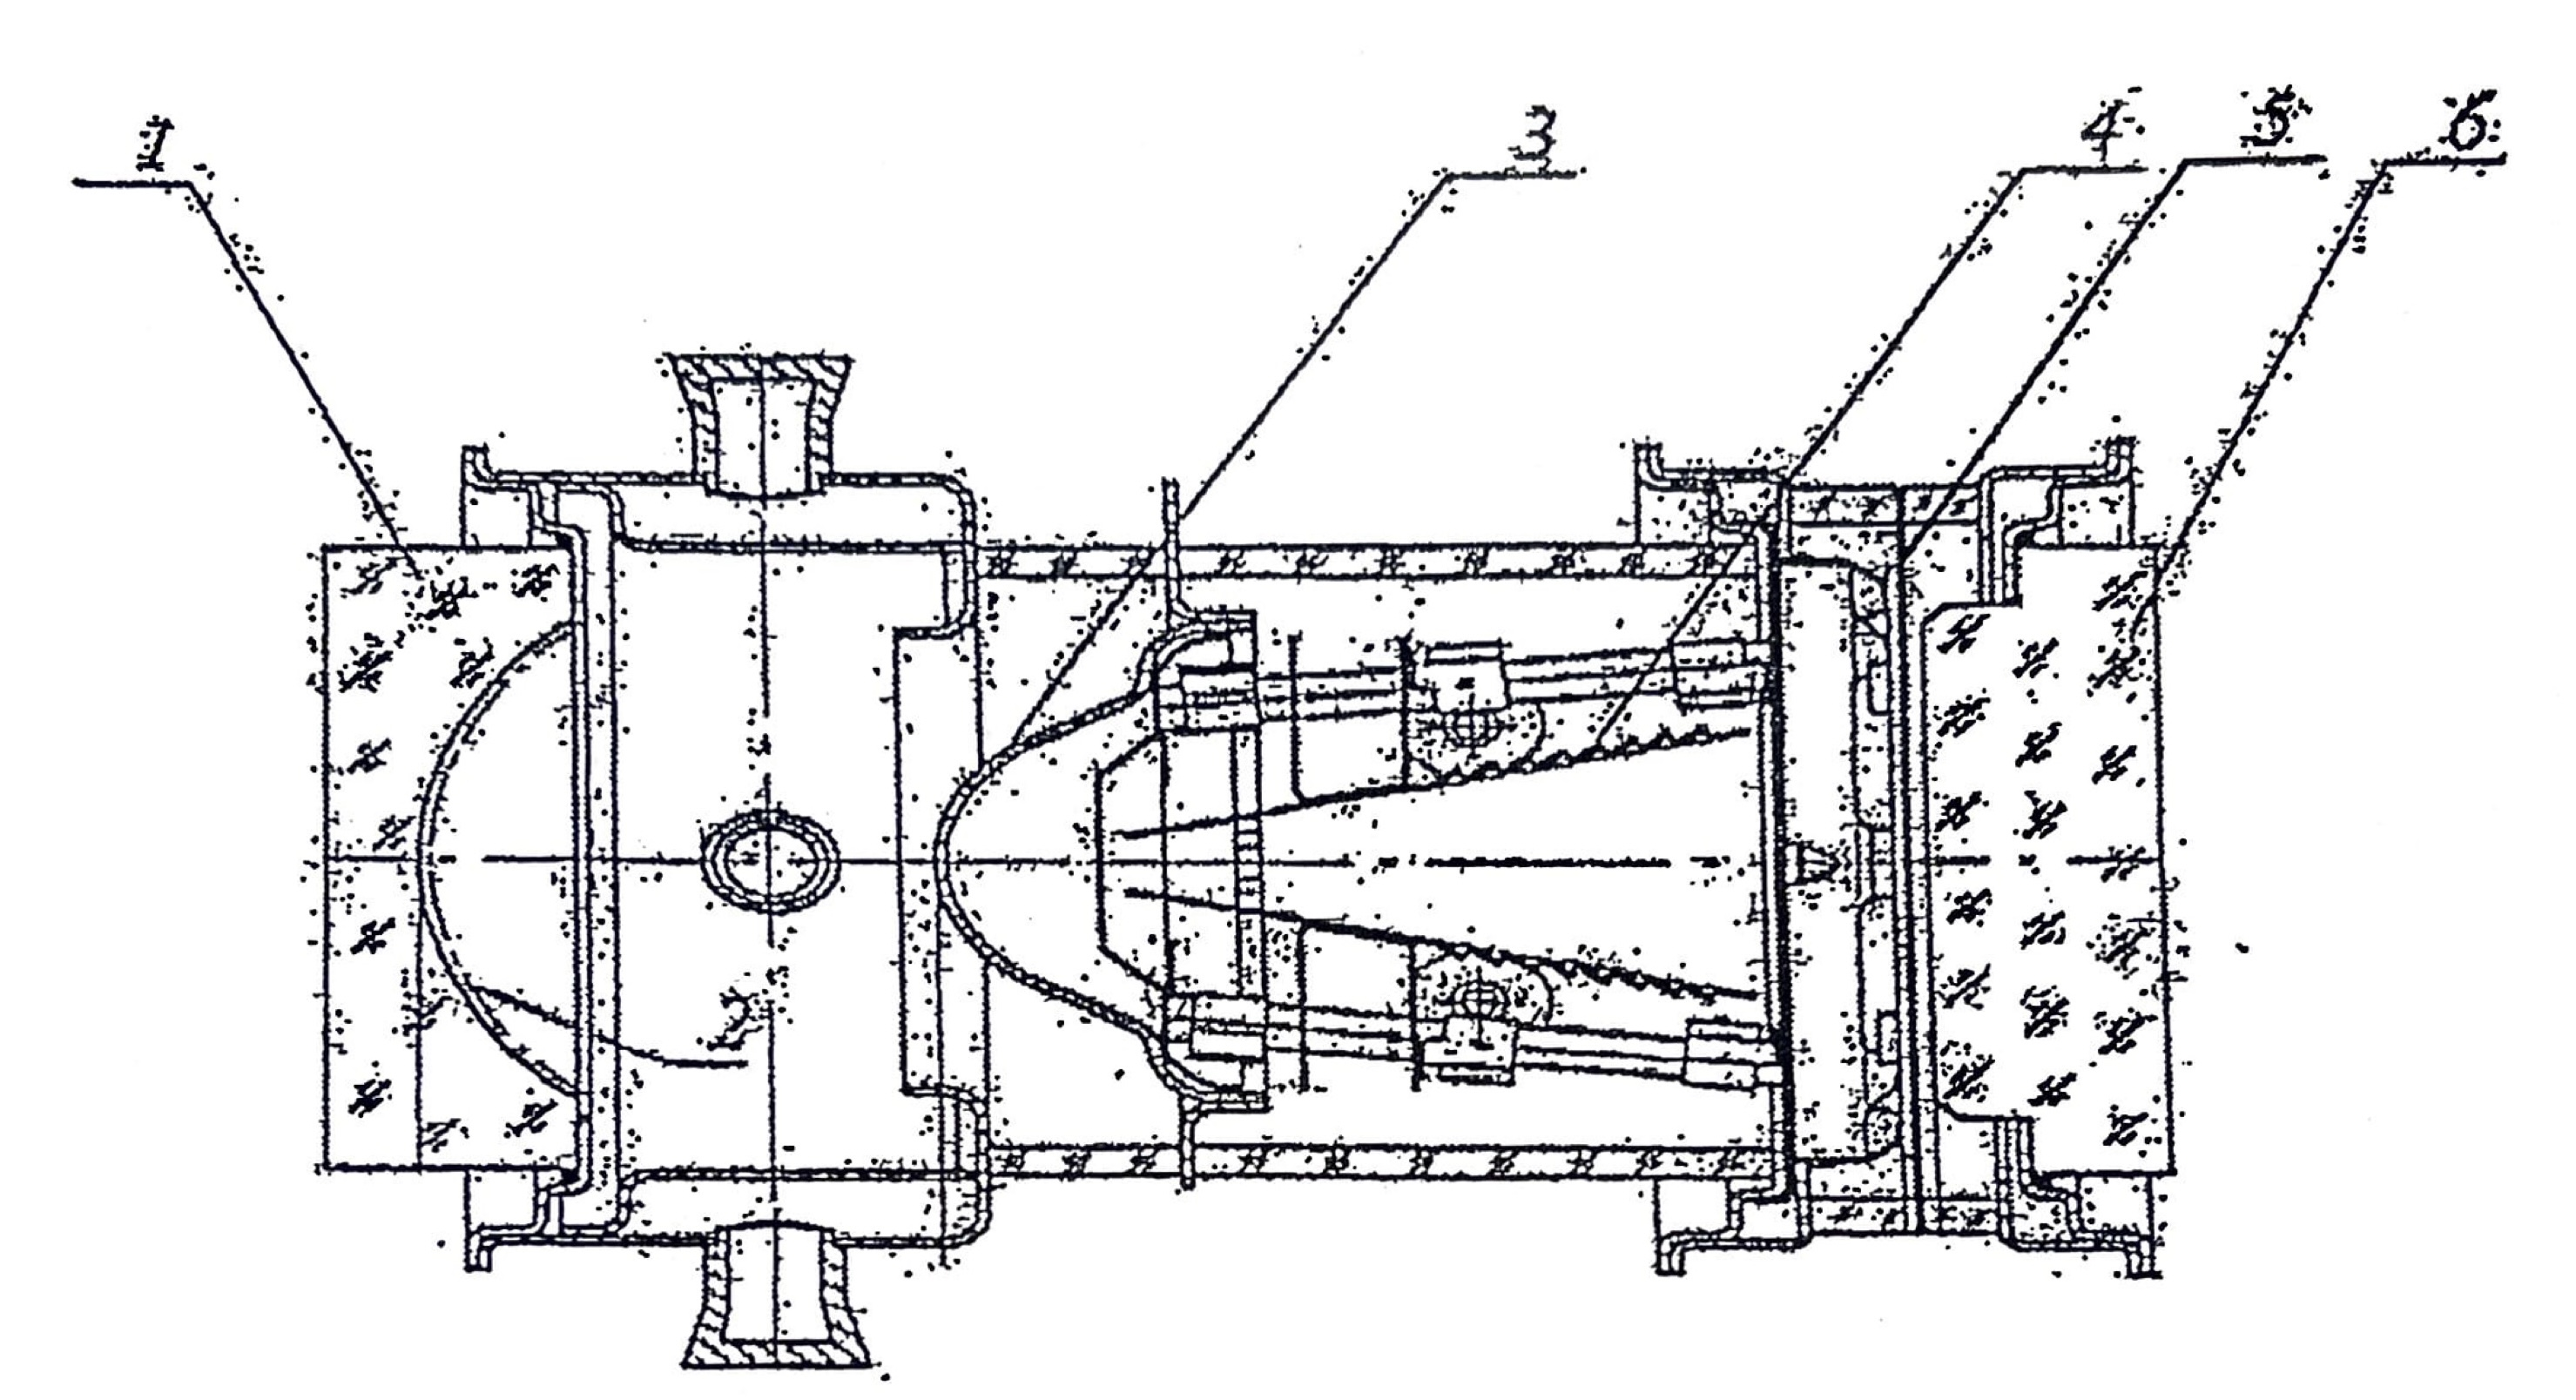
\includegraphics[width=350pt]{IMG_8962.png}
    \caption{Схема установки электронно-оптического преобразователя. 1 - стекловолоконное входное напряжение, 2 - фотокатод, 3 - анод, 4 - отклоняющие пластины, 5 - микроканальная пластина, 6 - выходное стекловолоконное окно}
    \label{установка}
\end{figure}
Входное оптическое излучение подается на фотокатод, изготовленный на стекловолоконной шайбе. Каждое волокно транспортирует оптическое излучение с входной плоскости ЭОП к фоточувствительному слою фотокатода. Когда налетающий электрон попадает в канал, то из стенки канала выбиваются вторичные электроны, которые ускоряются электрическим полем вдоль канала. Электрическое поле внутри канала создаётся путём приложения напряжения между поверхностями МКП. Экран покрыт люминофором, который при электронном возбужден обеспечивает свечение в зеленой области видимого спектра. Изображение на экране регистрируется с помощью видеокамеры.


\section* {Результаты измерений и обработка данных}

\subsection* {Подготовка экспериментальной установки}
Приводим установку в рабочее состояние. При помощи ручек можно регулировать напряжение катода, напряжение экрана и напряжение МКП; регистрировать ток анода, катода, МКП и экрана. По умолчанию значения напряжений МКП, экрана и катода равны 1.2 кВ, 3.5 кВ и 3.5 кВ соответственно.

% \subsection* {4.2. Измерения при постоянных напряжениях на МКП и экране}
% При значениях напряжения на экране и МКП по умолчанию меняем напряжение на катоде от 0.9 кВ до 4.2 кВ и фиксируем значения всех токов. Занесем полученные данные в таблицу

% \begin{table}[h!]
% \centering
% \begin{tabular}{|l|l|l|l|l|l|l|}
% \hline
% $U_{mkp}$,   кВ & $I_a$, мкА & $I_k$, мкА & $I_{mkp}$, мкА & $I_{scr}$, мкА & $U_k$, кВ & $U_{scr}$, кВ \\ \hline
% 1,52            & 3,27       & 0,01       & 6,48           & 0,00           & 1,99      & 3,51          \\ \hline
% 1,52            & 3,27       & -0,01      & 6,48           & 0,01           & 2,38      & 3,51          \\ \hline
% 1,52            & 3,25       & 0,02       & 6,48           & 0,00           & 2,80      & 3,51          \\ \hline
% 1,52            & 3,27       & 0,01       & 6,47           & 0,00           & 3,21      & 3,51          \\ \hline
% 1,52            & 3,27       & 0,01       & 6,48           & 0,00           & 3,60      & 3,51          \\ \hline
% 1,52            & 3,27       & 0,05       & 6,47           & 0,00           & 4,00      & 3,51          \\ \hline
% \end{tabular}
% \caption{Результаты измерений при фиксированных значениях напряжения на микроканальной пластине $U_{mkp}$ и напряжения на экране $U_{scr}$}
% \end{table}

% Построим график зависимости $I_{k}$ от напряжений на катоде, на МКП и на экране:

% \begin{center}
%     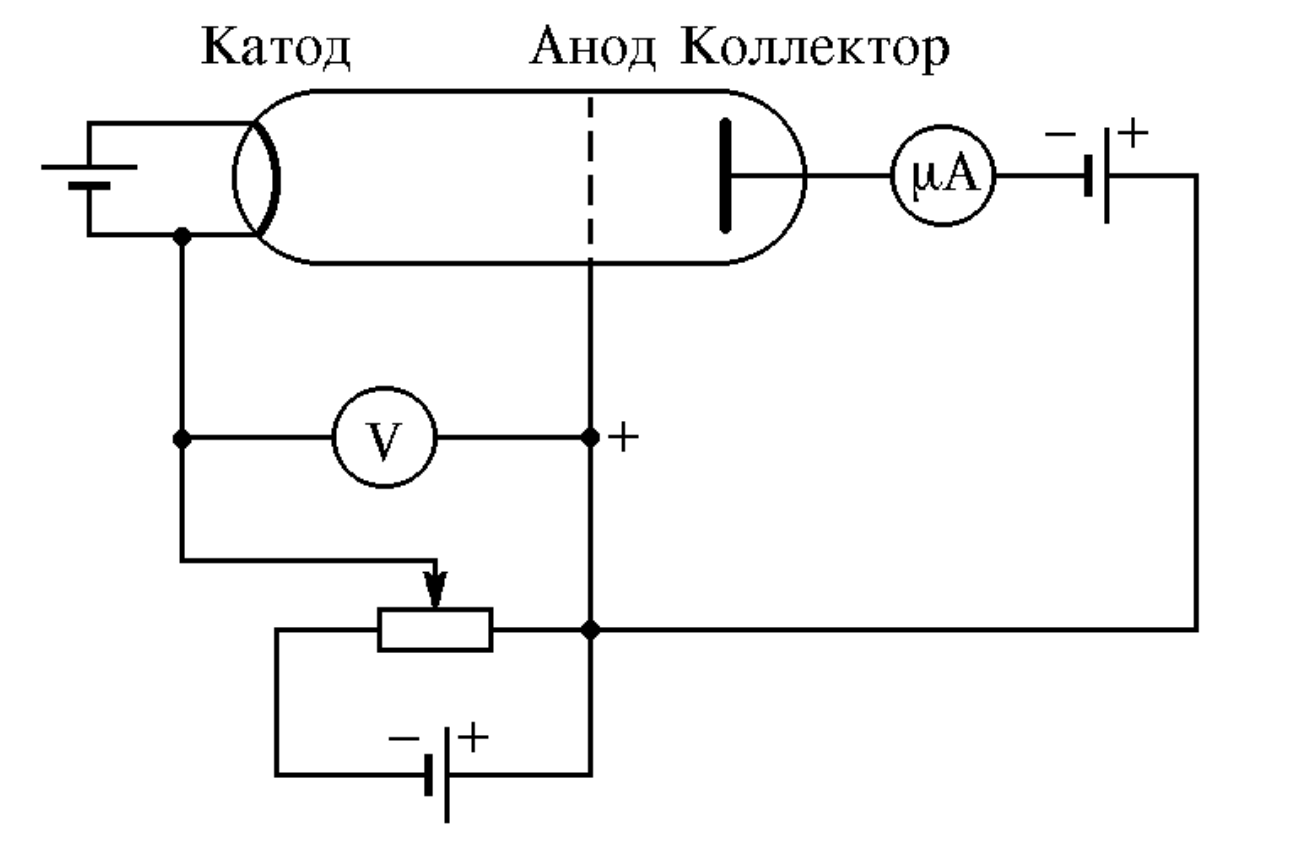
\includegraphics[scale = 1]{1.png}
%     \captionof{figure}{График зависимости $I_{k}$ от напряжений на катоде, на МКП и на экране}
% \end{center}

\subsection* {Измерения при постоянных напряжениях на катоде и экране}

При значениях напряжения на экране и катоде по умолчанию меняем напряжение на МКП от 0.5 кВ до 1.5 кВ и фиксируем значения всех токов. Запишем полученные данные в таблицу \ref{1}:

\begin{table}[h]
\centering
\begin{tabular}{|c|c|c|c|c|c|c|}
\hline
$U_{k}$, кВ & $U_{mkp}$, кВ & $U_{scr}$, кВ & $I_{k}$, мкА & $I_{mkp}$, мкА & $I_{scr}$, мкВ & $I_{a}$, мкА \\ \hline
3,48     & 0,51  & 3,49  & 0,02  & 2,08  & 0,01  & 1,04 \\ \hline
3,48     & 0,6   & 3,49  & 0,02  & 2,44  & 0,01  & 1,22 \\ \hline
3,48     & 0,7   & 3,49  & 0,02  & 2,85  & 0,01  & 1,44 \\ \hline
3,48     & 0,8   & 3,49  & 0,02  & 3,29  & 0,01  & 1,65 \\ \hline
3,48     & 0,9   & 3,49  & 0,02  & 3,68  & 0,01  & 1,86 \\ \hline
3,48     & 1,0     & 3,49  & 0,02  & 4,13  & 0,01  & 2,08 \\ \hline
3,48     & 1,1   & 3,49  & 0,02  & 4,54  & 0,01  & 2,3  \\ \hline
3,48     & 1,2   & 3,49  & 0,02  & 5,00     & 0,01  & 2,51 \\ \hline
3,48     & 1,3   & 3,49  & 0,02  & 5,42  & 0,01  & 2,72 \\ \hline
3,48     & 1,4   & 3,49  & 0,02  & 5,90   & 0,01  & 2,97 \\ \hline
3,48     & 1,5   & 3,49  & 0,02  & 6,38  & 0,01  & 3,22 \\ \hline
\end{tabular}
\caption{Результаты измерений при фиксированных значениях напряжения на катоде $U_{k}$ и напряжения на экране $U_{scr}$}
\label{1}
\end{table}

Построим график зависимости $I_{{mkp}}$ и $I_{a}$ от $U_{mkp}$ (остальные токи при этом не изменялись):

\begin{figure}[h]
    \centering
    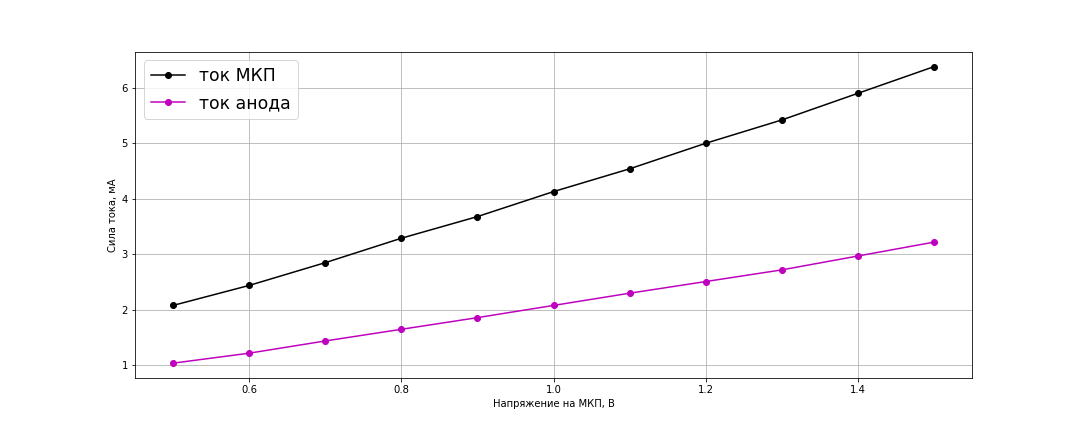
\includegraphics[width=0.99\textwidth]{2 pic.png}
    \caption{График зависимости $I_{{mkp}}(U_{mkp})$ и $I_{a}(U_{mkp})$}
\end{figure}

\subsection* {Измерения при постоянных напряжениях на катоде и МКП}

Варьируя напряжение на катоде от 2 до 4 кВ, фиксируем значения всех токов. Ни одна величина существенно не отклонялась от этих значений:

\begin{table}[h]
\centering
\begin{tabular}{|l|l|l|l|l|l|l|}
\hline
$U_{mkp}$,   кВ & $I_a$, мкА & $I_k$, мкА & $I_{mkp}$, мкА & $I_{scr}$, мкА & $U_k$, кВ & $U_{scr}$, кВ \\ \hline
1,52            & 3,27       & 0,01       & 6,47           & 0,00           & 3,50      & 2,01          \\ \hline
% 1,52            & 3,28       & -0,01      & 6,49           & 0,01           & 3,50      & 2,41          \\ \hline
% 1,52            & 3,29       & 0,02       & 6,46           & 0,00           & 3,50      & 2,83          \\ \hline
% 1,52            & 3,27       & 0,01       & 6,49           & 0,00           & 3,50      & 3,21          \\ \hline
% 1,52            & 3,28       & 0,01       & 6,49           & 0,00           & 3,50      & 3,61          \\ \hline
% 1,52            & 3,28       & 0,05       & 6,48           & 0,00           & 3,50      & 3,84          \\ \hline
\end{tabular}
\end{table}

% Построим график зависимости $I_{scr}$ от напряжений на МКП, на экране и на катоде:

% \begin{center}
%     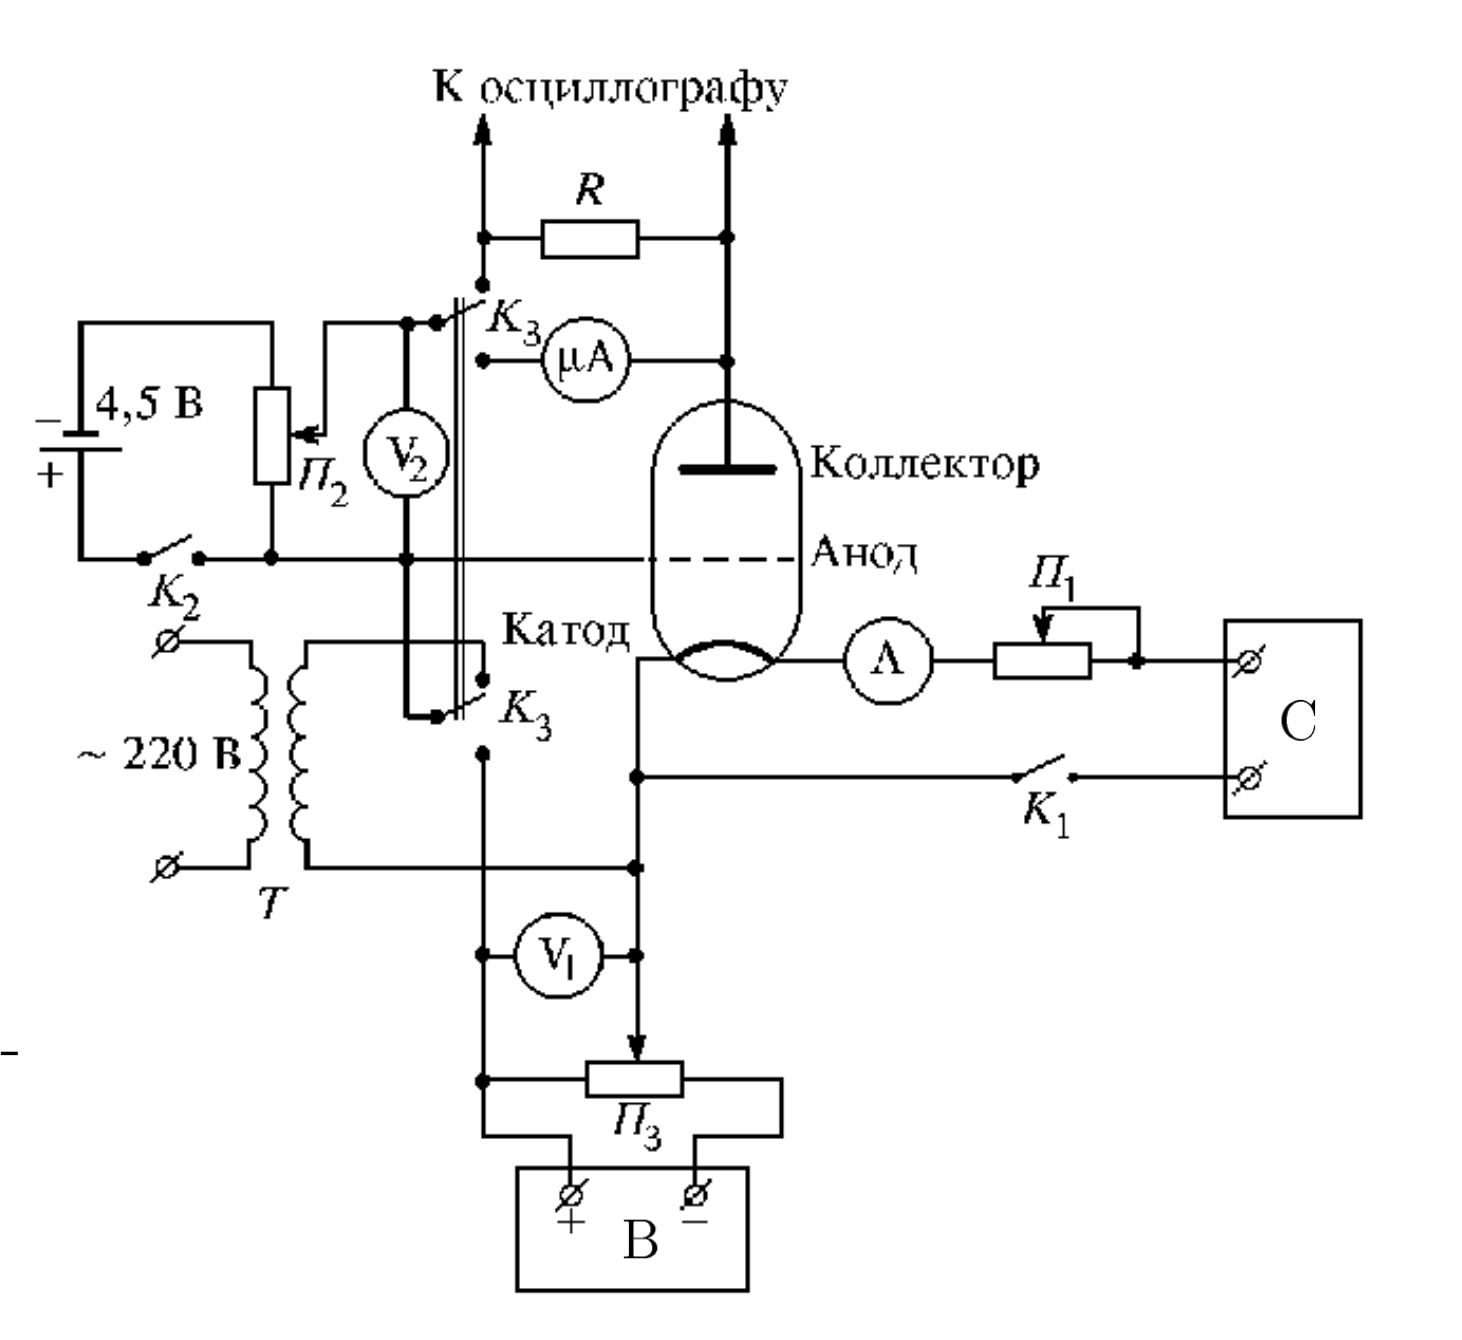
\includegraphics[scale = 1]{3.png}
%     \captionof{figure}{График зависимости $I_{scr}$ от напряжений на МКП, на экране и на катоде}
% \end{center}

\subsection* {Изменение яркости изображения при помощи светофильтров}

Устанавливая различные цветные светофильтры, зарегистрируем изменение тока катода, анода, МКП и экрана при фиксированных напряжениях: $U_{scr} = 3,5$ кВ, $U_{k} = 3,5$ кВ, $U_{mkp} = 1,2$ кВ. Пронаблюдаем изменение яркости изображения.

\begin{center}
    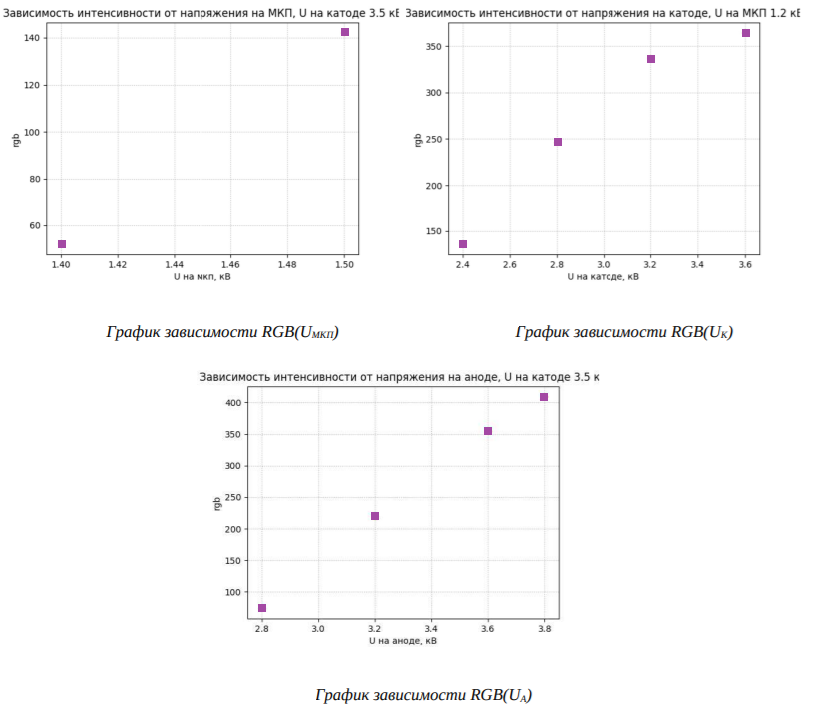
\includegraphics[scale = 1]{3 pic.png}
    % \captionof{figure}{графики зависимост $I_{{mkp}}(U_{mkp})$ и $I_{a}(U_{mkp})$}
\end{center}

Таким образом мы из обширного спектра излучения, падающего на фотокатод выделяли лишь свет определенной длины волны. Результаты представлены в таблице ниже:

\begin{table}[t]
\centering
\begin{tabular}{|c|c|c|c|c|}
\hline
Светофильтр & Цвет            & R  & G  & B  \\ \hline
СС15        & фиолетовый      & 10  & 20 & 17 \\ \hline
СЗС9        & сине-фиолетовый & 6  & 21 & 17 \\ \hline
СЗС17       & синий           & 20 & 65 & 49 \\ \hline
СЗС23       & голубой         & 27 & 77 & 61 \\ \hline
ЖС10        & зеленый         & 33 & 93 & 72 \\ \hline
ЖС19        & салатовый       & 32 & 87 & 67 \\ \hline
ЖС18        & желто-оранжевый & 17 & 67 & 47 \\ \hline
ОС12        & оранжевый       & 11 & 34 & 24 \\ \hline
КС10        & красный         & 6  & 11 & 10 \\ \hline
ПС7         & пурпурный       & 21 & 64 & 50 \\ \hline
\end{tabular}
\end{table}

В таблице указаны интенсивности красной, зеленой и синей составляющей в изображении сетки на экране. Благодаря ним можно судить и об интенсивности излучения той или иной длины волны в спектре.

Из таблицы видно, что пик интенсивности приходится на зеленый свет. Также можно заметить, что интенсивность красного света очень низкая, но интенсивность пурпурного довольно высока, из чего можно сделать вывод, что еще один пик интенсивности находится вблизи синего света. Таким образом, спектр состоит преимущественно из света с длиной волны от 450 до 600 нм, с пиками в области 	460 и 550 нм, что соответствует табличным данным.

\section*{Вывод}

В данной работе мы ознакомились с устройством электронно-оптического преобразователя, исследовали зависимости силы тока на катоде, аноде, МКП и экране от напряжений на этих же элементах. В итоге получили линейные зависимости силы тока на аноде и МКП от напряжения на МКП (см. рис.4). На опыте убедились, что картинка становилась ярче с увеличением напряжения.

Также с помощью светофильтров был исследован спектр излучения света, падающего на фотокатод. Благодаря полученным данным мы пришли к выводу, что спектр преимущественно состоит из света с длиной волны 450-600 нм с пиками, приходящимися на излучение с длиной волны 460нм и 550нм, т.е. синий и зеленый свет соответственно, что соответствует табличным данным.


\end{document}
